%! Author = lazza
%! Date = 28/05/2022

\section{MIMD}\label{sec:mimd}
The execution can be synchronous or asynchronous, deterministic or non-deterministic.

\paragraph{Advantages:} \textbf{Multipurpose} processor that can be built starting from \textbf{standard CPUs} (often
off-the-shelf
microprocessors) that act independently one from the other: each processor fetches its own instructions and operates
on its own data.
\textbf{Scalable} to a variable number of processor nodes.\\
\textbf{Flexible:}
\begin{itemize}
    \item single-user machines focusing on high-performance for one
    specific application
    \item multi-programmed machines running many tasks
    simultaneously
    \item some combination of these functions.
\end{itemize}
\textbf{Cost/performance} advantages due to the use of off-
the-shelf microprocessors these can be combined in the same system.

\paragraph{Disadvantage:} Fault tolerance issues.

\paragraph{Exploting MIMD} To exploit a MIMD with $n$ processors, we need:
\begin{itemize}
    \item at least $n$ threads or processes to execute
    \item independent threads typically identified by the programmer or
    created by the compiler
    \item parallelism is contained in the threads \textrightarrow thread-level parallelism
\end{itemize}

\textbf{Note:} parallelism is identified by the software.\\

\subsection{Memory architecture}\label{subsec:memory-architecture}
Existing MIMD machines fall into 2 classes, depending on the number
of processors involved, which in turn dictates a memory organization
and interconnection strategy.

\paragraph{Key design issues}
\begin{itemize}
    \item how many processors?
    \item how powerful are processors?
    \item how do parallel processors share data?
    \item where to place the physical memory?
    \item how do parallel processors cooperate and coordinate?
    \item what type of interconnection topology?
    \item how to program processors?
    \item how to maintain cache coherency?
    \item how to maintain memory consistency?
    \item how to evaluate system performance?
\end{itemize}

\subsubsection{Centralized shared-memory architectures}\label{subsubsec:centralized-shared-memory-architectures}
\begin{itemize}
    \item at most few dozen processor chips (< 100 cores)
    \item large caches, single memory multiple banks
    \item often called symmetric multiprocessors (SMP) and the
    style of architecture called Uniform Memory Access (UMA), see section~\ref{subsec:bus-based-symmetric-shared-memory}
\end{itemize}

\begin{figure}[h]
    \centering
    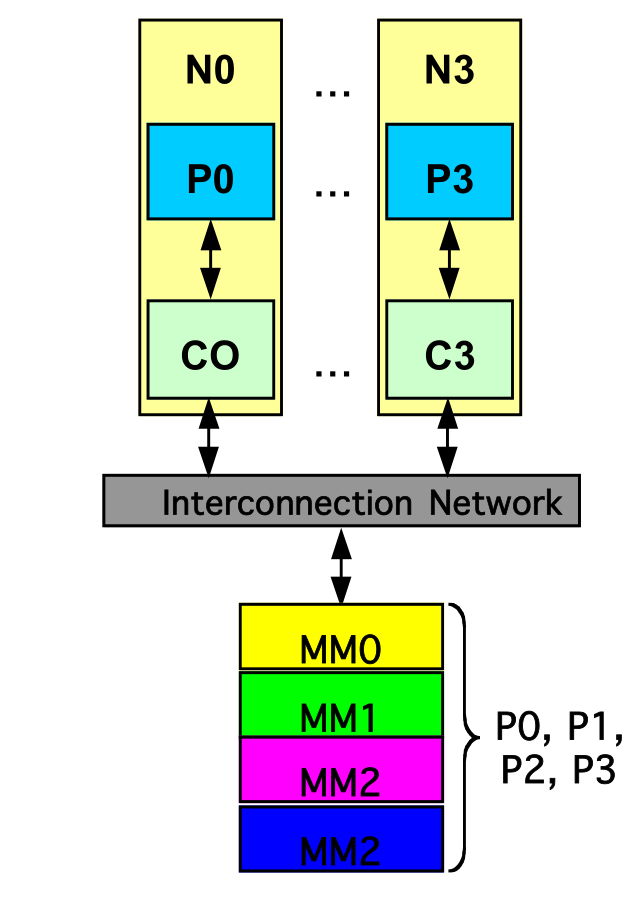
\includegraphics[scale = 0.2]{images/centralized-shared-memory-architectures}
    \caption{Shared memory architecture}
    \label{fig:centralized-shared-memory-architectures}
\end{figure}

\subsubsection{Distributed memory architectures}\label{subsubsec:distributed-memory-architectures}
\begin{itemize}
    \item to support large processor counts
    \item requires high-bandwidth interconnect
    \item disadvantage: need of data communication among processors
    \item Non Uniform Memory Access (NUMA)
\end{itemize}

\begin{figure}[h]
    \centering
    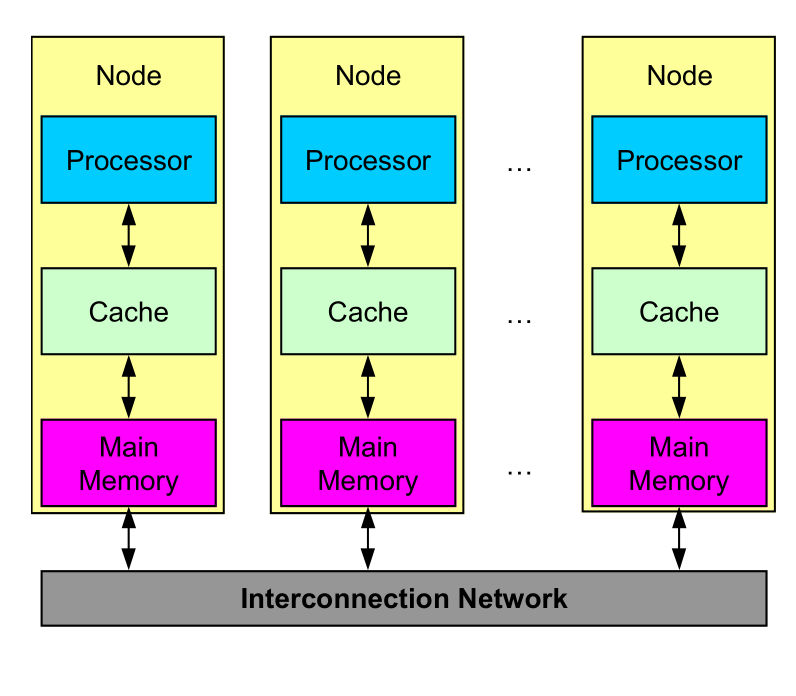
\includegraphics[scale = 0.2]{images/distributed-memory-architectures}
    \caption{Distributed memory architectures}
    \label{fig:distributed-memory-architectures}
\end{figure}

\paragraph{Tile64} is a VLIW ISA multicore processor manufactured by Tilera.
It consists of a mesh network of 64 "tiles", where each tile houses a general purpose processor, cache,
and a non-blocking router, which the tile uses to communicate with the other tiles on the processor.
The short-pipeline, in-order, three-issue cores implement a MIPS-inspired VLIW instruction set.
Each core has a register file and three functional units: two integer arithmetic logic units and a load-store unit.
Each of the cores ("tile") has its own L1 and L2 caches plus an overall virtual L3 cache which is an aggregate of all
the L2 caches.
A core is able to run a full operating system on its own or multiple cores can be used to run a symmetrical
multi-processing operating system.

\begin{figure}[h]
    \centering
    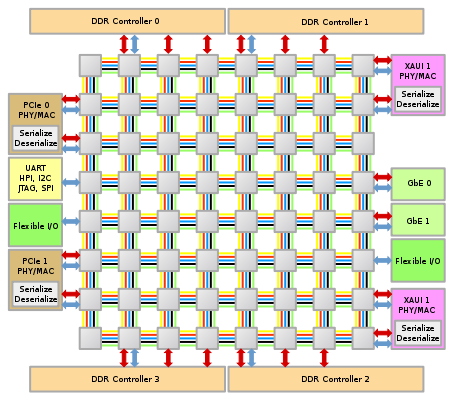
\includegraphics[scale = 0.4]{images/Tile64}
    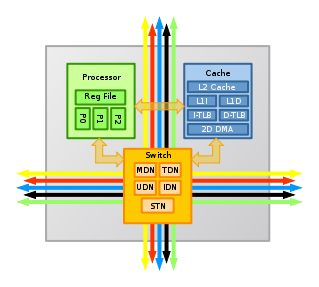
\includegraphics[scale = 0.5]{images/Tile64-Tile}
    \caption{Tile64}
    \label{fig:tile64}
\end{figure}


\subsubsection{Examples}\label{subsubsec:examples}

\paragraph{Cell: PS3}
Cell is a heterogeneous chip multiprocessor:
\begin{itemize}
    \item One 64-bit Power core
    \item 8 specialized co-processors\\
    \textrightarrow based on a novel single-instruction multiple-data (SIMD)
    architecture called SPU (Synergistic Processor Unit)
\end{itemize}

\paragraph{Xenon: XBOX360}
Xenon is a homogeneous chip multiprocessor:
\begin{itemize}
    \item three symmetrical cores, each two way SMT-capable and clocked at 3.2 GHz
    \item SIMD: VMX128 extension for each core
    \item 1 MMB L2 cache (lockable by the GPU) running at half-speed (1.6 GHz) with a 256-bit bus
\end{itemize}

Microsoft envisions a procedurally rendered game
as having at least two primary components:
\begin{itemize}
    \item Host thread: a game's host thread will contain the main
thread of execution for the game
    \item Data generation thread: where the actual procedural
synthesis of object geometry takes place
\end{itemize}
These two threads could run on the same PPE, or
they could run on two separate PPEs.
In addition to the these two threads, the game
could make use of separate threads for handling
physics, artificial intelligence, player input, etc.


\subsection{Procedural synthesis}\label{subsec:procedural-synthesis}
Procedural synthesis about making optimal use of system bandwidth
and main memory by dynamically generating lower-level geometry
data from statically stored higher-level scene data.

\begin{figure}[h]
    \centering
    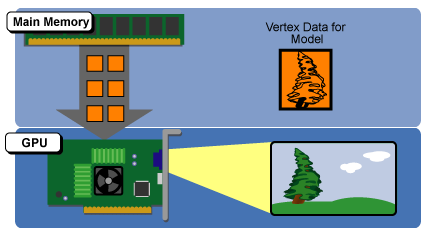
\includegraphics[scale = 0.]{images/procedural-synthesis}
    \caption{Procedural synthesis}
    \label{fig:procedural-synthesis}
\end{figure}

For 3D games:
\begin{itemize}
    \item Artists use a 3D rendering program to produce content for the game
    \item Each model is translated into a collection of polygons
    \item Each polygons is represented in the computer's memory as collections of vertices
\end{itemize}
When the computer is rendering a scene in a game in real-time:
\begin{itemize}
    \item Models that are being displayed on the screen start out in main
memory as stored vertex data
    \item That vertex data is fed from main memory into the GPU where it is then rendered into a 3D image and output
    to the monitor as a sequence of frames.
\end{itemize}

\paragraph{Limitations} there are two problems:
\begin{itemize}
    \item The costs of creating art assets for a 3D game are
going through the roof along with the size and
complexity of the games themselves
    \item Console hardware's limited main memory sizes and
limited bus bandwidth
\end{itemize}


\subsection{Memory Address Space Model}\label{subsec:memory-address-space-model}
How do parallel processors share data?
We already talked about how the physical memory implementation divides the \textit{machines} in two classes, now we 
look how the virtual memory is from the perspective of a process.

\subsubsection{Single logically shared address space}
A memory reference can be made by any processor to any memory location, this model adapts well to the
\textit{shared memory architectures}: the address space is shared among processors, the same physical address on 2
processors refers to the same location in memory.

\begin{figure}[h]
    \centering
    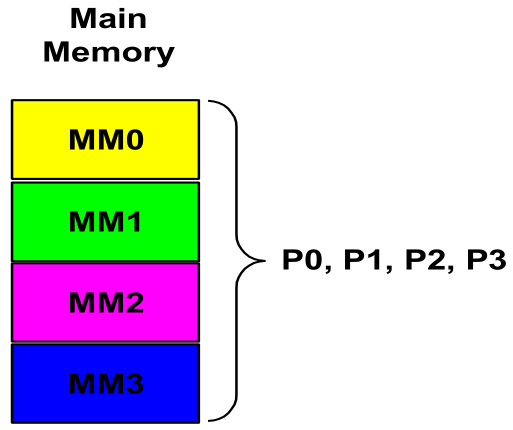
\includegraphics[scale = 0.3]{images/single-logically-shared-address-space}
    \caption{Single logically shared address space}
    \label{fig:single-logically-shared-address-space}
\end{figure}

\paragraph{Shared Address}
\begin{itemize}
    \item the processors communicate among them through shared variables in memory
    \item implicit management of the communication through load/store operations to access any memory locations
    \item shared memory does not mean that there is a single centralized memory
\end{itemize}

\subsubsection{Multiple and private address spaces}
The processors communicate among them through send/receive primitives, this model adapts well to \textit{message
passing architectures}: the address space is logically disjoint and cannot be addressed by different processors, the
same physical address on 2 processors refers to 2 different locations in two different memories.

\begin{figure}[h]
    \centering
    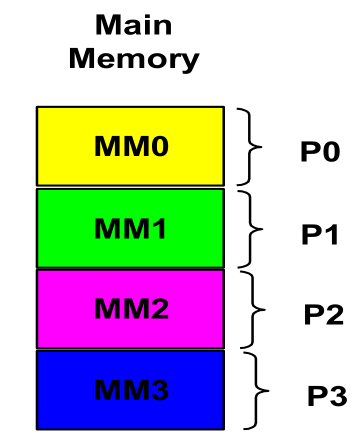
\includegraphics[scale = 0.3]{images/multiple-and-private-address-spaces}
    \caption{Multiple and private address spaces}
    \label{fig:multiple-and-private-address-spaces}
\end{figure}

\paragraph{Private address}
\begin{itemize}
    \item the processors communicate among them through sending/receiving messages
    \item explicit management of the communication through send/receive primitives to access private memory locations
    \item no cache coherency problem among processors
\end{itemize}

\textbf{Note:} The concepts of addressing space
(single/multiple) and the physical memory
organization (centralized/distributed) are
orthogonal to each other: they could be combined freely.
Multiprocessor systems can have single
addressing space and distributed physical
memory.

\begin{figure}[h]
    \centering
    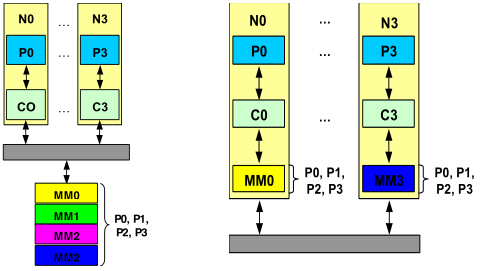
\includegraphics[scale = 0.43]{images/address-space-vs-physical-memory-org}
    \caption{Single shared space vs physical memory}
    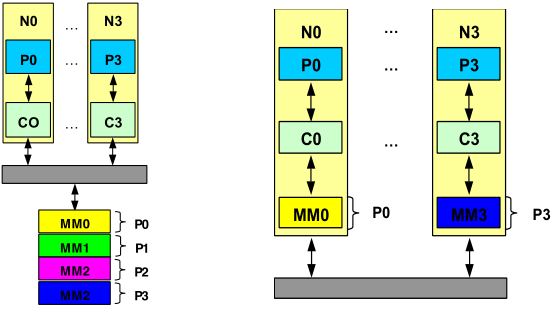
\includegraphics[scale = 0.40]{images/address-space-vs-physical-memory-org-1}
    \caption{Multiple private addresses vs physical memory }
    \label{fig:address-space-vs-physical-memory-org}
\end{figure}


\subsection{Programming Model}\label{subsec:programming-model}

\subsubsection{Shared Memory}
The program is a collection of threads of control, each thread:
\begin{itemize}
    \item can be created dynamically, mid execution, in some languages.
    \item has a set of \textit{private} variables, e.g., local stack variables
    \item also a set of \textit{shared} variables, e.g., static variables, shared common blocks, or global heap
\end{itemize}

Processes communication:
\begin{itemize}
    \item implicitly by writing and reading shared variables
    \item coordination by synchronizing on shared variables
\end{itemize}

\begin{figure}[h]
    \centering
    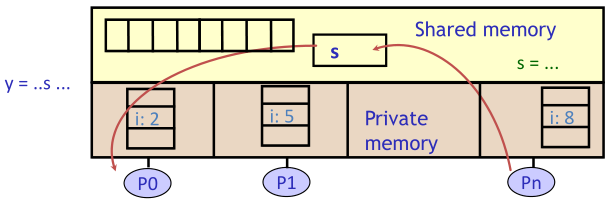
\includegraphics[width = \linewidth]{images/shared-memory-model}
    \caption{Shared memory}
    \label{fig:shared-memory-model}
\end{figure}

\paragraph{Advantages}
\begin{itemize}
    \item implicit communication (loads/stores)
    \item low overhead when cached
\end{itemize}

\paragraph{Disadvantages}
\begin{itemize}
    \item complex to build in way that scales well -- e.g., distance between core and memory may become too much
    cutting down performance
    \item requires synchronization operations
    \item hard to control data placement within caching system
\end{itemize}

\subsubsection{Message Passing}
The program consist of a collection of \textbf{named} processes:
\begin{itemize}
    \item usually fixed at program startup time
    \item thread of control plus local address space, no shared data
    \item logically shared data is partitioned over local processes
\end{itemize}

Processes communication:
\begin{itemize}
    \item explicitly by send/receive pairs
    \item coordination is implicit in every communication event
    \item MPI (Message Passing Interface) is the most commonly used SW
\end{itemize}

\begin{figure}[h]
    \centering
    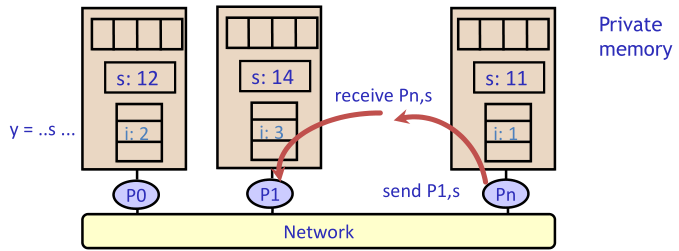
\includegraphics[width = \linewidth]{images/message-passing-model}
    \caption{Message passing}
    \label{fig:message-passing-model}
\end{figure}

\paragraph{Advantages}
\begin{itemize}
    \item explicit communication (sending/receiving of messages)
    \item easier to control data placement (no automatic caching)
\end{itemize}

\paragraph{Disadvantages}
\begin{itemize}
    \item message passing overhead can be quite high
    \item more complex to program
    \item introduces question of reception technique (interrupts/polling)
\end{itemize}

\paragraph{Massively Parallel Processors Problems}
\begin{itemize}
    \item all data must be handled by software: cannot retrieve remote data except with message request/reply
    \item message passing has high software overhead:
    \begin{itemize}
        \item early machines had to invoke OS on each message
        \item even user level access to network interface has dozens of cycle overhead
        \item sending messages can be cheap (just like stores)
        \item receiving messages is expensive, need to poll or interrupt
    \end{itemize}
\end{itemize}

\subsection{Bus-based symmetric shared memory}\label{subsec:bus-based-symmetric-shared-memory}
The most popular architecture till now sees each core and its own cache memory, with a simple networking solution, the
bus, which connects processors with each other and to the shared memory.

\textbf{Note:} here we refer to \textit{physical} shared memory architecture (UMA).

\begin{figure}[h]
    \centering
    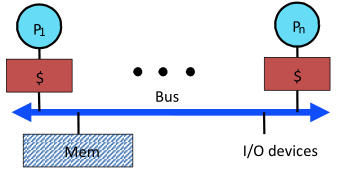
\includegraphics[scale = 0.45]{images/bus-based-symmetric-shared-memory}
    \caption{Bus-based symmetric multiprocecessors}
    \label{fig:bus-based-symmetric-shared-memory}
\end{figure}

Attractive as throughput servers and for parallel programs:
\begin{itemize}
    \item Fine-grain resource sharing
    \item Uniform access via loads/stores
    \item Automatic data movement and coherent replication in caches
    \item Cheap and powerful extension
\end{itemize}
It uses the normal uni-processor mechanisms to access data, the key to make it viable is the extension of memory
hierarchy to support multiple processors.

\paragraph{Shared memory machines} Two main categories:
\begin{itemize}
    \item non cache coherent
    \item hardware cache coherent
\end{itemize}
Will work with any data, but might be slow, we can choose to optimize only critical portions of code.
Load and store instructions used to communicate data: no OS involvement \textrightarrow low software overhead.
Usually there are some special synchronization primitives.
In large scale systems, the logically distributed shared memory is implemented as physically distributed memory
modules.\footnote{Some notions might be wrong in this section, double check}

\subsection{Cache coherence}\label{subsec:cache-coherence}
Shared memory architectures cache both \textbf{private data}, used by a single processor, and \textbf{shared data},
used by multiple processors to provide communication.
When shared data is cached, the shared valued may be replicated in multiple caches.
In addition to the reduction in access latency and required memory bandwidth, this replication provides a reduction
of shared data contention when multiple processors have to read simultaneously the same data.
Private processors caches create a problem:
\begin{itemize}
    \item copies of a variable can be present in multiple caches
    \item a write by one processor may not become visible to others
\end{itemize}
The use of multiple copies of the same data introduces a new problem: cache coherency.

\paragraph{Writing policies}
When a system writes data to cache, it must at some point write that data to the backing store as well.
The timing of this write is controlled by what is known as the write policy.
There are two basic writing approaches:
\begin{itemize}
    \item \textbf{write-through}: write is done synchronously both to the cache and to the backing store
    \item \textbf{write-back} (also called write-behind): initially, writing is done only to the cache.
    The write to the backing store is postponed until the modified content is about to be replaced by another cache block.
\end{itemize}

\begin{figure}[h]
    \centering
    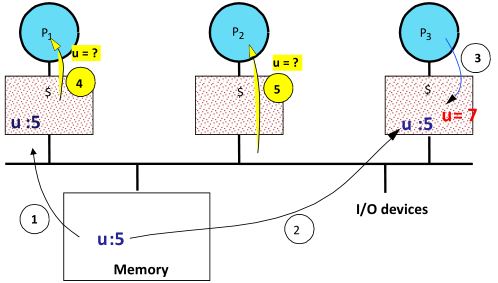
\includegraphics[scale = 0.4]{images/cache-coherence-problem}
    \caption{Cache coherence problem}
    \label{fig:cache-coherence-problem}
\end{figure}
\textbf{Note:} processors see different values for $u$ after event 3.
With write back caches, the value written back to memory depends on which cache flushes or writes back values first:
processes accessing main memory may see very stale value.

\paragraph{What does coherency means}
Informal definition: \textit{"any read must return the most recent write} \textrightarrow too strict and difficult to
implement.\\
A better definition: \textit{any write must eventually be seen by a read}, all write are seen in \textbf{serialized
order}, that is two write to the same location by any two processors are seen in the same order by all processors
plus the latest (in time) will be seen (in memory).
If P writes x and P1 reads it, P’s write will be seen by P1 if the read
and write are sufficiently far apart and no other writes to x occur
between the two accesses: \textbf{propagation of writes} after a certain amount of time.

\paragraph{When a written value will be seen?}
We cannot require that a read of x by P1 can
instantaneously see the write of x by another
processor that precedes by a small amount of time.
This is a problem of \textbf{memory consistency}, coherency and consistency are complementary:
\begin{itemize}
    \item coherence defines the behavior of reads and writes to the same memory location
    \item consistency defines the behavior of reads and write with respect to accesses to other memory locations
\end{itemize}
Assumptions for now:
\begin{itemize}
    \item a write does not complete (and allow the next write to occur) until all processors have seen the effect of
    that write
    \item the processor does not change the order of any write with respect to any other memory access
\end{itemize}

\paragraph{Coherent caches}
A program running on multiple processors will normally
have copies of the same data in several caches.
In a coherent multiprocessor the caches provide both
\textbf{migration} and \textbf{replication} of shared data items:
\begin{itemize}
    \item Migration: a data item can be moved to a local cache
    and used there in a transparent fashion, reduces both the latency to access a shared data item that
    is allocated remotely and the \textit{bandwidth demand} on the shared memory
    \item Replication for shared data that are being
    simultaneously read: caches make a copy of the data
    item in the local cache, reduces both latency of access and \textit{contention for a shared read}
\end{itemize}

\paragraph{Potential solutions} HW-based solutions to maintain coherency: cache-coherence protocols.
Key issue: implement a cache coherent protocol in multiprocessors needs tracking the status of any sharing of a data
block.
Two classes of protocols:
\begin{itemize}
    \item snooping protocols
    \item directory-based protocols
\end{itemize}


\subsubsection{Snooping Protocols}
\begin{itemize}
    \item[\textrightarrow] All cache controllers monitor (snoop) on the bus to
    determine whether or not they have a copy of the block
    requested on the bus and respond accordingly.
    \item[\textrightarrow] Every cache that has a copy of the shared block, also
    has a copy of the sharing status of the block, and no
    centralized state is kept.
    \item[\textrightarrow]
    Send all requests for shared data to all processors.
    \item [\textrightarrow] Require broadcast, since caching info is at processors.
    \item [\textrightarrow] Suitable for Centralized Shared-Memory Architectures,
    and in particular for small scale multiprocessors with
    single shared bus.
\end{itemize}

\paragraph{Snoopy cache Goodman 1983}
Idea: have cache watch (or snoop upon) DMA\footnote{Direct Memory Access}, and then \textit{do the right thing}.
Snoopy caches tags are dual-ported:

\begin{figure}[h]
    \centering
    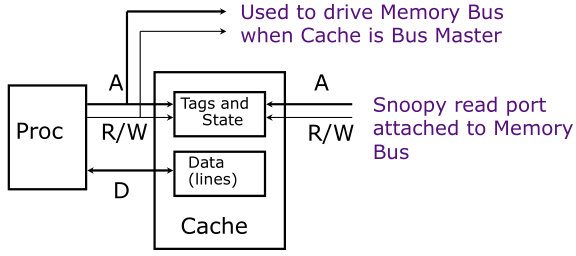
\includegraphics[scale = 0.4]{images/snoopy-cache-goodman}
    \caption{Snoopy cache goodman}
    \label{fig:snoopy-cache-goodman}
\end{figure}

Bus is a broadcast medium and caches know what
they have.
Cache controller “snoops” all transactions on the
shared bus:
\begin{itemize}
    \item relevant transaction if the cache contains that block
    \item take action to ensure coherence (\textrightarrow invalidate, update, or supply value):
    \subitem depends on state of the block and the protocol
\end{itemize}


